\documentclass[tikz, border=5mm]{standalone}

\usetikzlibrary{arrows.meta,decorations.markings,fit,calc, positioning}

\definecolor{componentColor}{RGB}{210,210,210}
\definecolor{systemColor}{RGB}{230,230,230}

\tikzset{component/.append style={fill=componentColor, align=center, draw, minimum width=2cm, minimum height=1.5cm, rounded corners=.3cm}}
\tikzset{system/.style={component, fill=systemColor, rounded corners=0cm}}
\tikzset{interface/.style={system, fill=systemColor, minimum size=1.6cm}}

\tikzstyle{arrow} = [-{Latex[scale=3.0]}]
\tikzset{arrowLabel/.append style={minimum height=.25cm, draw=none}}
\begin{document}

	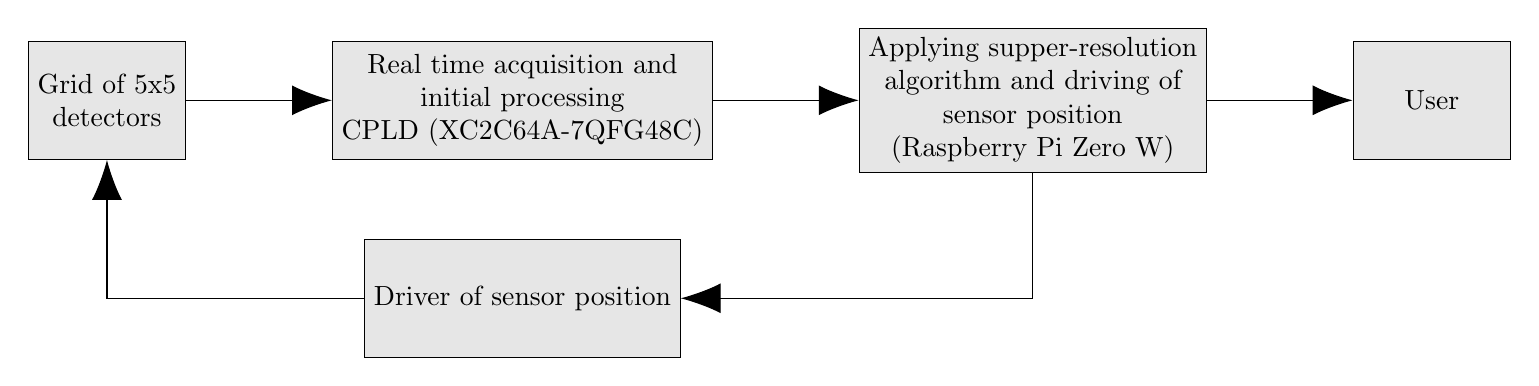
\begin{tikzpicture}[node distance=1.0cm and 1.85cm]
	% Nodes
	\pgfdeclarelayer{background}
	\pgfsetlayers{background,main}
		\node (detectors) [system] {Grid of 5x5 \\ detectors};
		\node (acquisition) [system, right=of detectors] {Real time acquisition and\\initial processing\\ CPLD (XC2C64A-7QFG48C)};
        \node (processing) [system, right=of acquisition] {Applying supper-resolution\\ algorithm and driving of \\ sensor position\\ (Raspberry Pi Zero W)};
		\node (motor) [system, below=of acquisition] {Driver of sensor position};
		\node (user) [system, right=of processing] {User};

		% Connectors
		\begin{scope}[->]
            \draw [arrow] (detectors) -- (acquisition);
            \draw [arrow] (acquisition) -- (processing);
			\draw [arrow] (processing.south) -| ++(0,0)  |- node[anchor=north, minimum width=.25cm, draw=none]{{}}  (motor.east);
			\draw [arrow] (motor.west) -| ++(0,0)  -| node[anchor=south, minimum width=.25cm, draw=none]{{}}  (detectors.south);
			\draw [arrow] (processing) -- (user);
	    \end{scope}
\end{tikzpicture}
\end{document}
